\chapter{Manual de usuario}
\label{sec:manual}

El manual de usuario se va a realizar para una máquina ubuntu.\\

\section{Instalación de Docker}

Para guardar mejor las modificaciones que se vayan realizando es mejor instalar una máquina docker en lugar de hacerlo en local. Así el primer paso es instalar la última versión de docker, en esta parte se seguirá el tutorial oficial de Docker \cite{instalacion-docker}. Antes de nada se va a desinstalar cualquier versión anterior de Docker, código \ref{cod:remove-docker}\\

\begin{lstlisting}[language=Bash,caption=Instalación Docker. Parte I, label=cod:remove-docker, style=Consola]
	$ sudo apt-get remove docker docker-engine docker.io containerd runc
\end{lstlisting}


Es necesario actualizar los paquetes \texttt{apt} para tener acceso a las últimas actualizaciones e instalar los paquetes que permiten al sistema operativo acceder a los repositorios de Docker a través de HTTPS, código \ref{cod:docker-up}.\\

\begin{lstlisting}[language=Bash,caption=Instalación Docker. Parte II, label=cod:docker-up, style=Consola]
	$ sudo apt-get update
	$ sudo apt-get install apt-transport-https ca-certificates curl gnupg-agent software-properties-common
\end{lstlisting}

Se añade la clave GPG oficial de Docker, código \ref{cod:add-huella}. La clave GPG es una característica de seguridad para asegurar que el software que se va instalar es auténtico.\\
 
\begin{lstlisting}[language=Bash,caption=Instalación Docker. Parte III, label=cod:add-huella, style=Consola]
	$ curl -fsSL https://download.docker.com/linux/ubuntu/gpg | sudo apt-key add -

	OK
\end{lstlisting}

Verificar que obtenemos la clave con la siguiente huella, para ello hay que buscar la huella con los últimos 8 dígitos, de la misma, código \ref{cod:huella}.\\

\texttt{9DC8 5822 9FC7 DD38 854A  E2D8 8D81 803C 0EBF CD88}\\

\begin{lstlisting}[language=Bash,caption=Instalación Docker. Parte IV, label=cod:huella, style=Consola]
	$ sudo apt-key fingerprint 0EBFCD88

	pub   rsa4096 2017-02-22 [SCEA]
		  9DC8 5822 9FC7 DD38 854A  E2D8 8D81 803C 0EBF CD88
	uid           [ unknown] Docker Release (CE deb) <docker@docker.com>
	sub   rsa4096 2017-02-22 [S]
\end{lstlisting}

La instalación del repositorio de Docker se hace mediante el código \ref{cod:install-docker}.\\ 

\begin{lstlisting}[language=Bash,caption=Instalación Docker. Parte V, label=cod:install-docker, style=Consola]
	$ sudo add-apt-repository "deb [arch=amd64] https://download.docker.com/linux/ubuntu $(lsb_release -cs) stable"
\end{lstlisting}

Actualizar los repositorios que se acaban de agregar, e instalar la última versión de Docker Engine y Docker Containerd, código \ref{cod:docker-update}.\\

\begin{lstlisting}[language=Bash,caption=Instalación Docker. Parte VI, label=cod:docker-update, style=Consola]
	$ sudo apt-get update
	$ sudo apt-get install docker-ce docker-ce-cli containerd.io
\end{lstlisting}

Verificar que se ha instalado correctamente comprobando la versión de Docker, código \ref{cod:docker-version}.\\

\begin{lstlisting}[language=Bash,caption=Instalación Docker. Parte VII, label=cod:docker-version, style=Consola]
	$ docker --version

	Docker version 19.03.13, build 4484c46d9d
\end{lstlisting}

Algunos comandos útiles para el trabajo con Docker se muestran en el código \ref{cod:cm-docker}.\\

\begin{lstlisting}[language=Bash,caption=Comandos útiles de Docker, label=cod:cm-docker]
	#Muestra los contenedores
	$ sudo docker ps

	#Lista los contenedores con los IDs
	$ sudo docker container ls --all

	#Lista las imagenes con los IDs
	$ sudo docker images ls --all 

	#Guarda los cambios del docker
	$ sudo docker commit <ID-CONTAINER> <NOMBRE-NUEVO:ETIQUETA>

	#Corre un contenedor, abriendo los puertos indicados
	$ sudo docker run -it -p <PUERTO:PUERTO> <NOMBRE:ETIQUETA>

	#Elimina un contenedor
	$ sudo docker rm <ID-CONTAINER>
\end{lstlisting}

\section{Instalación Blockchain ARK}

En Docker, hay que iniciar una imagen de ubuntu xenial, código \ref{cod:run-docker}. Además es necesario abrir algunos puertos como 4103, para la API pública, 4102, conexión P2P API y 4200, para el \textit{explorer}.\\

\begin{lstlisting}[language=Bash,caption=Instalación \textit{blockchain}. Parte I, label=cod:run-docker, style=Consola]
	$ sudo docker run -ti -p 4102:4102 -p 4103:4103 -p 4200:4200 ubuntu:xenial
\end{lstlisting}

Una vez dentro de la máquina Docker hay que instalar \texttt{sudo}, para poder trabajar en modo administrador desde el usuario que se va a crear, código \ref{cod:add-user}.\\

\begin{lstlisting}[language=Bash,caption=Instalación \textit{blockchain}. Parte II, label=cod:add-user, style=Consola]
	$ apt-get update
	$ apt-get install sudo
	$ adduser deployer

	Añadiendo el usuario `deployer' ...
	Añadiendo el nuevo grupo `deployer' (1001) ...
	Añadiendo el nuevo usuario `deployer' (1001) con grupo `deployer' ...
	Creando el directorio personal `/home/deployer' ...
	Copiando los ficheros desde `/etc/skel' ...
	Introduzca la nueva contraseña de UNIX: ********
	Vuelva a escribir la nueva contraseña de UNIX: ********
	passwd: contraseña actualizada correctamente
	Cambiando la información de usuario para deployer
	Introduzca el nuevo valor, o presione INTRO para el predeterminado
		Nombre completo []: 
		Número de habitación []: 
		Teléfono del trabajo []: 
		Teléfono de casa []: 
		Otro []: 
	¿Es correcta la información? [S/n] S
\end{lstlisting}

Cambiar el modo del usuario \texttt{``{}}deployer\texttt{''}, incluyéndolo en el grupo sudo, para que sea un superusuario y finalmente, entrar al usuario deployer, código \ref{cod:enter-user}.\\

\begin{lstlisting}[language=Bash,caption=Instalación \textit{blockchain}. Parte III, label=cod:enter-user, style=Consola]
	$ usermod -aG sudo deployer
	$ su - deployer
\end{lstlisting}

Actualizar los paquete e instalar algunos nuevos como \texttt{git}, \texttt{curl} y \texttt{yarn}, código \ref{cod:update}.\\

\begin{lstlisting}[language=Bash,caption=Instalación \textit{blockchain}. Parte IV, label=cod:update, style=Consola]
	$ sudo apt-get update
	$ sudo apt-get install git curl jq apt-transport-https nano
\end{lstlisting}

Instalar las dependencias \texttt{nvm}, código \ref{cod:nvm}, es necesario para instalar posteriormente el paquete \texttt{pm2}.\\

\begin{lstlisting}[language=Bash,caption=Instalación \textit{blockchain}. Parte V, label=cod:nvm, style=Consola]
	$ curl -o- https://raw.githubusercontent.com/creationix/nvm/v0.33.8/install.sh | bash
\end{lstlisting}

Para comprobar que se ha instalado correctamente hay que salir y volver a entrar en el usuario \texttt{``{}}deployer\texttt{''}, código \ref{cod:verif-nvm}.\\

\begin{lstlisting}[language=Bash,caption=Instalación \textit{blockchain}. Parte VI, label=cod:verif-nvm, style=Consola]
	$ exit
	$ su - deployer
	$ command -v nvm

	nvm
\end{lstlisting}

Si en algún momento se desea desinstalar la dependencia \texttt{nvm} habrá que seguir los comandos \ref{cod:remove-nvm}.\\

\begin{lstlisting}[language=Bash,caption=Instalación \textit{blockchain}. Parte VII, label=cod:remove-nvm, style=Consola]
	$ nvm use system
	$ npm uninstall -g a_module
	$ sudo npm  install -g npm
\end{lstlisting}

Para instalar pm2 ver el código \ref{cod:npm}.\\

\begin{lstlisting}[language=Bash,caption=Instalación \textit{blockchain}. Parte VIII, label=cod:npm, style=Consola]
	$ sudo apt-get install npm
	$ sudo npm i -g pm2
	$ sudo ln -s /usr/bin/nodejs /usr/bin/node
\end{lstlisting}

Algunos comandos interesantes para trabajar con pm2 se muestran en el código \ref{cod:pm2}. Servirán para observar si la \textit{blockchain} y el \textit{explorer} están levantados.\\

\begin{lstlisting}[language=Bash,caption=Comandos útiles de pm2, label=cod:pm2, style=Consola]
	#Lista los demonios de pm2
	$ pm2 list

	#Se obtienen los estados de los demonios de pm2
	$ pm2 status
\end{lstlisting}

Hasta aquí se han instalado los paquetes y dependencias para poder empezar a instalar la \textit{blockchain}. Ahora hay que clonar el directorio deployer de \texttt{@ArkEcosystem}, código \ref{cod:clone-ark}.\\

\begin{lstlisting}[language=Bash,caption=Instalación \textit{blockchain}. Parte IX, label=cod:clone-ark, style=Consola]
	$ git clone https://github.com/ArkEcosystem/deployer.git
	$ chmod 764 deployer/setup.sh
	$ ./deployer/setup.sh
\end{lstlisting}


Una vez instalado el deployer hay que proceder a realizar una modificación en el archivo \path{/home/<USUARIO>/deployer/app/app-core.sh}, código \ref{cod:app-core-A}. Para que en lugar de instalar el repositorio de github sin modificaciones, se instale la \textit{blockchain} con el nuevo algoritmo UOV.\\

\begin{lstlisting}[language=Python,caption=Línea 108 app-core.sh, label=cod:app-core-A]
	git clone https://github.com/mvictoria1997/core.git --single-branch "$BRIDGECHAIN_PATH"
\end{lstlisting}

La \textit{blockchain} va a utilizar la base de datos local del Docker, así pues hay que iniciarla con el código \ref{cod:start-sql}. Además va a ser necesario instalar la librería \texttt{libjemalloc} para no tener problemas de memoria.\\

\begin{lstlisting}[language=Bash,caption=Instalación \textit{blockchain}. Parte X, label=cod:start-sql, style=Consola]
	$ sudo service postgresql start
	$ sudo apt-get update -y 
	$ sudo apt-get install -y libjemalloc-dev
\end{lstlisting}

Durante la instalación de la \textit{blockchain} se descargará el código con los algoritmos de firma, por tanto en este punto debemos de modificar los archivos. Para ello hay que hacer un \texttt{fork} del repositorio \texttt{ArkEcosystem/core} \cite{ark-core} en nuestro usuario de Github. A continuación se descarga el código con el comando \ref{cod:clone-core}.\\

\begin{lstlisting}[language=Bash,caption=Clonar nuevo core, label=cod:clone-core, style=Consola]
	$ git clone https://github.com/<USUARIO>/core.git
\end{lstlisting}

Los archivos que se van a modificar se encuentran en el directorio \path{core/packages/src/crypto/hash.ts}. En el archivo \texttt{hash.ts} se modifican las funciones de firma y verificación con el algoritmo ECDSA quedando de la forma que muestra el código \ref{cod:hash-ECDSA}.\\


Se añaden, en el archivo \texttt{hash.ts}, las funciones de firma y validación de la misma con el algoritmo UOV. Ver código \ref{cod:hash-UOV-sign} para la firma y código \ref{cod:hash-UOV-verif} para la verificación.\\



Hay que añadir los archivos en \texttt{python} a donde se realizarán las llamadas desde \texttt{typescript}. Estos son los ficheros \texttt{signature.py} para la firma, código \ref{cod:sign-py} y \texttt{verify.py} para la validación, código \ref{cod:veri-py}.\\




Finalmente se crean los dos ficheros \texttt{.json}, en ellos se puede incluir un ejemplo para ver que estructura van a seguir dichos archivos. \\

El código \ref{cod:data-json} muestra un ejemplo de la estructura del fichero \texttt{data.json} que almacena las claves privadas y públicas tanto para el algoritmo de Schnorr como para el de UOV.\\

\begin{lstlisting}[language=Python,caption=Ejemplo fichero \texttt{data.json}, label=cod:data-json]
	[
		{"id":1,
			"pub_schnorr": "D2",
			"priv_schnorr":"C6",
			"priv_alpha_UOV": [[1, 0 ], [ 1, 1]],
			"priv_beta_OUV": [1, 0,  1],
			"pub_alpha_UOV": [[1,  1], [ 0, 1]],
			"pub_beta_OUV": [[1, 0,  1, 1, 1]]
		}
	]
\end{lstlisting}

El código \ref{cod:signature-json} muestra un ejemplo de la estructura del fichero \texttt{signatue.json} que almacena las firmas en dos formatos, hexadecimal y en vector.\\

\begin{lstlisting}[language=Python,caption=Ejemplo fichero \texttt{signature.json}, label=cod:signature-json]
	[
		{"hex":"54ga24",
		"vector":[[1,0,0,0,1],[1,0,1,0,1,0]]}
	]
\end{lstlisting}


Llegados a este punto hay que instalar el \texttt{core} de la \textit{blockchain} con el algoritmo UOV, código \ref{cod:install-bridgechain}, la instalación tardará unos diez minutos. Una vez que instalado se obtiene en la salida la dirección y la \textit{passphrase} del wallet Genesis, ambas serán necesarias para poder realizar transacciones por tanto puede resultar útil almacenarlas en un archivo, ver figura \ref{fig:install-bridge}. De todas formas se puede encontrar la \textit{passphrase} junto con la dirección en el archivo \path{/home/<USUARIO>/.bridgechain/testenet/<NOMBRE-BRIDGECHAIN>/genesisWallet.json}. \\

El archivo de configuración \path{/home/<USUARIO>/deployer/config.sample.conf} se puede modificar para cambiar por ejemplo el nombre de la \textit{blockchain}, en este caso se le ha puesto  \texttt{``{}}victoria-bridgechain\texttt{''}, variable \texttt{chainName}. Otros parámetros a destacar para modificar son \texttt{databaseName}, \texttt{totalPremine}, \texttt{bridgechainPath} y \texttt{explorerPath}.\\

\begin{itemize}
	\item \texttt{databaseName}: Nombre de la base de datos.
	\item \texttt{totalPremine}: El valor total de tokens o monedas que tendrá la red local.
	\item \texttt{bridgechainPath}: \textit{path} del directorio de instalación de la \textit{blockchain}.
	\item \texttt{explorerPath}: \textit{path} del directorio de instalación del \textit{explorer}.
\end{itemize}

\begin{lstlisting}[language=Bash,caption=Instalación \textit{blockchain}. Parte XI, label=cod:install-bridgechain, style=Consola]
	$ ./deployer/bridgechain.sh install-core --config deployer/config.sample.json --autoinstall-deps --non-interactive
\end{lstlisting}

\begin{figure}[H]
	\centering
	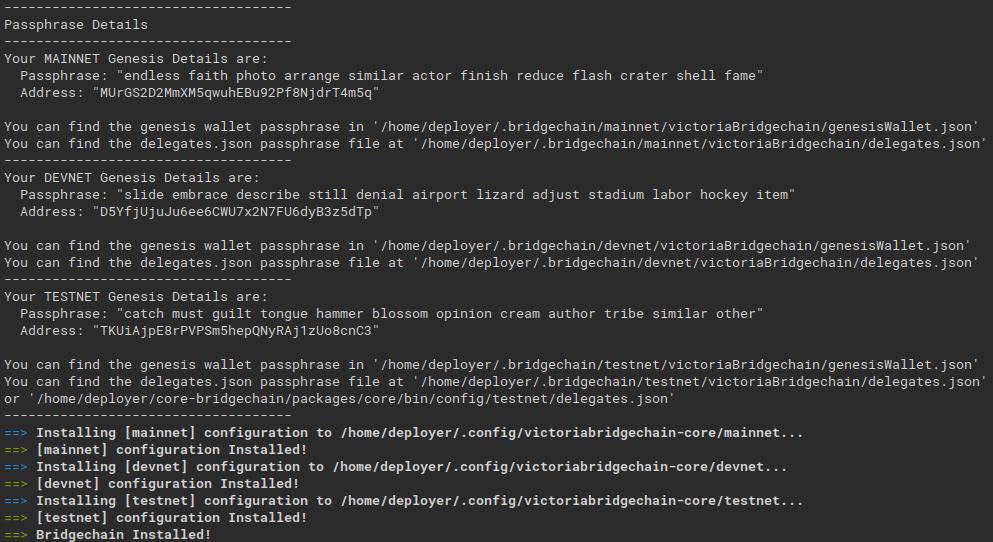
\includegraphics[width=15cm,height=9cm]{figuras/Instalacion_bridgechain.png}
	\caption{Salida tras la instalación del core}
	\label{fig:install-bridge}
\end{figure}

A continuación se instalará el \textit{explorer} para poder ver las transacciones y bloques generados, código \ref{cod:install-explorer}.\\

\begin{lstlisting}[language=Bash,caption=Instalación \textit{blockchain}. Parte XII, label=cod:install-explorer, style=Consola]
	$ ./deployer/bridgechain.sh install-explorer --config deployer/config.sample.json --skip-deps --non-interactive
\end{lstlisting}


El último paso es iniciar la \textit{blockchain} y el \textit{explorer}, código \ref{cod:start-brid}. La salida tras iniciar el \textit{explorer} la muestra la figura \ref{fig:install-explorer}, que son los estados de la \textit{blockchain} y del \textit{explorer}. Esto mismo se visualizar con el comando \texttt{pm2 status}.\\

\begin{lstlisting}[language=Bash,caption=Instalación \textit{blockchain}. Parte XIII, label=cod:start-brid, style=Consola]
	$ ./deployer/bridgechain.sh start-core --network testnet

	==> Starting...
	Starting victoriabridgechain-relay... done
	Starting victoriabridgechain-forger... done
	==> Start OK!


	$ ./deployer/bridgechain.sh start-explorer --network testnet
\end{lstlisting}


\begin{figure}[H]
	\centering
	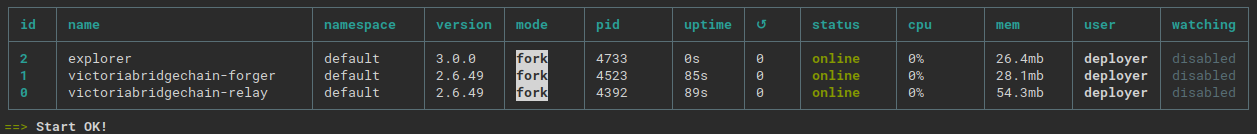
\includegraphics[width=12.5cm,height=1.5cm]{figuras/Instalacion_explorer.png}
	\caption{Salida tras iniciar del \textit{explorer}}
	\label{fig:install-explorer}
\end{figure}

Para visualizar las transacciones en el \textit{explorer}, debemos de abrir un navegador y acceder a la url \texttt{http://NODE\_GENESIS\_IP:EXPLORER\_PORT}, donde el \texttt{EXPLORER\_PORT} es $4200$. La figura \ref{fig:nav-explorer} muestra las primeras transacciones realizadas, entre ellas se encuentra la transacción inicial al monedero génesis, además del registro de los delegados.\\

\begin{figure}[H]
	\centering
	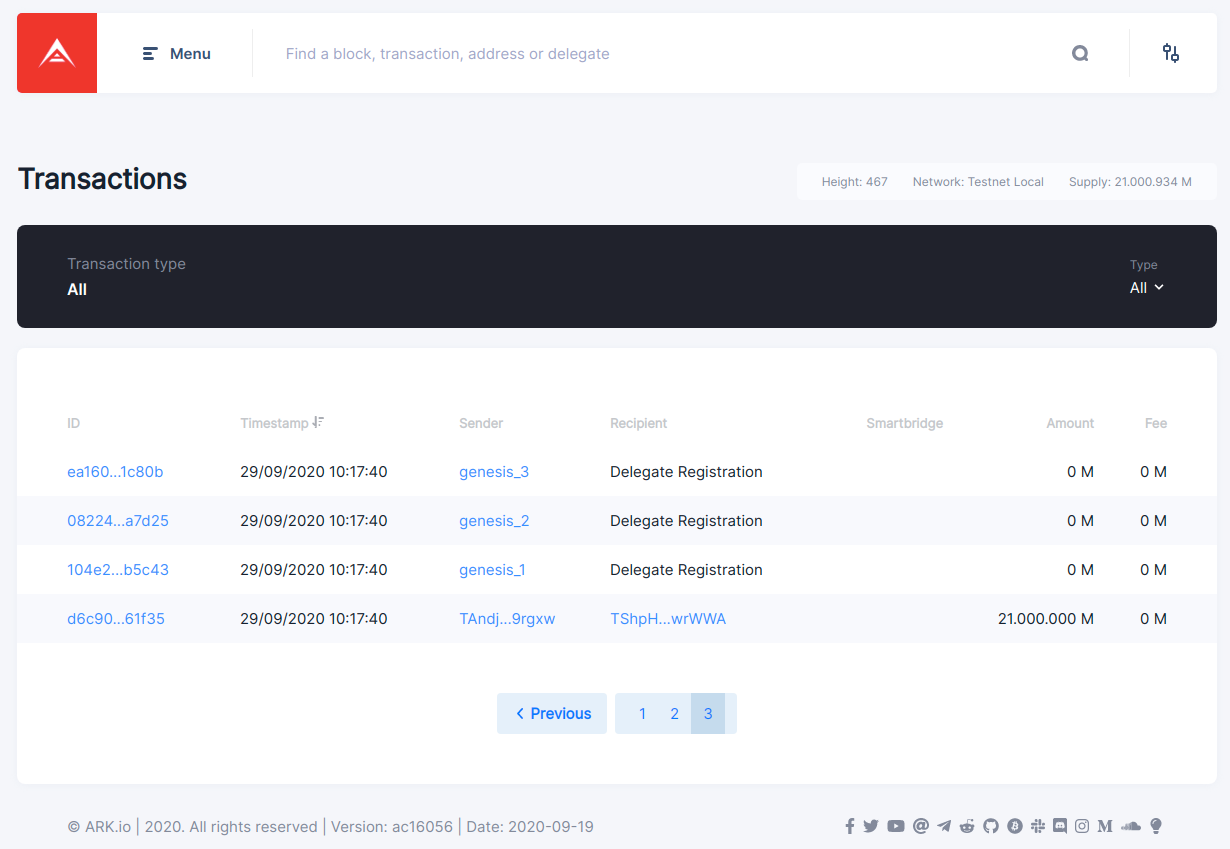
\includegraphics[width=11cm,height=7cm]{figuras/Navegacion_explorer.png}
	\caption{Primeras transacciones en el \textit{explorer}}
	\label{fig:nav-explorer}
\end{figure}


\newpage
\section{Instalación de la aplicación ARK Desktop Wallet}
\label{sec:manual-wallet}

Antes de descargar la aplicación ARK Desktop Wallet, en el ordenador local, son necesarias algunas instalaciones previas, como algunos archivos de desarrollo de \texttt{libudev}, \texttt{node 12} y \texttt{yarn}, código \ref{cod:install-wallet}.\\

\begin{lstlisting}[language=Bash,caption=Instalaciones previas a la aplicación ARK Wallet, label=cod:install-wallet, style=Consola]
$ sudo apt-get install libudev-dev libusb-1.0-0-dev

$ npm install -g n
$ sudo n 12

# Para comprobar que se ha instalado node 12
$ n --version

$ npm install -g yarn
\end{lstlisting}

La descarga de la aplicación se realiza desde el repositorio de github de \texttt{@ArkEcosystem/desktop-wallet} \cite{descargas-wallet}, para el proyecto se ha descargado la última versión del archivo \texttt{.deb}.\\

\begin{lstlisting}[language=Bash,caption=Instalación de la aplicación ARK Wallet, label=cod:install-wallet, style=Consola]
$ sudo dpkg -i ark-desktop-wallet-linux-amd64-<VERSION>.deb

#Para desintalarlo
$ sudo apt-get remove ark-desktop-wallet
\end{lstlisting}


Una vez que se ha instalado la aplicación, la abrimos y nos encontramos con la figura \ref{fig:wallet-1}. A continuación, vamos siguiendo los pasos que nos salen en la parte de la derecha de la pantalla.\\

\begin{figure}[H]
	\centering
	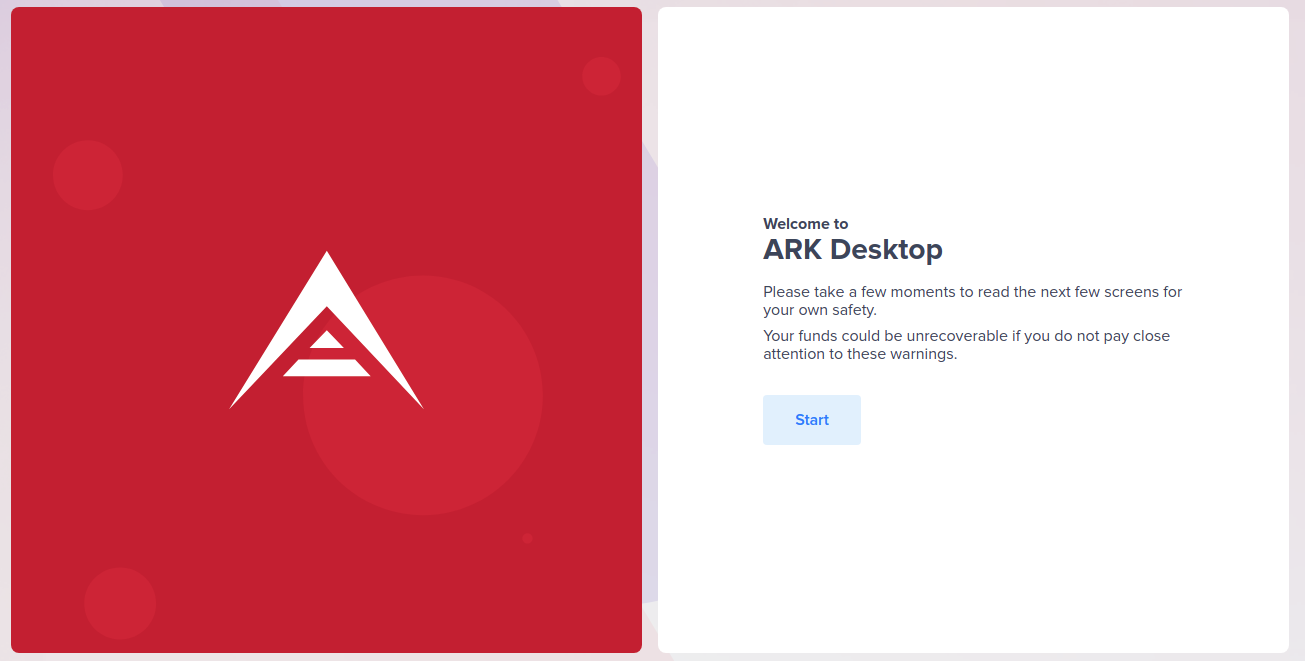
\includegraphics[width=12.5cm,height=6.5cm]{figuras/wallet_1.png}
	\caption{Inicio de Wallet}
	\label{fig:wallet-1}
\end{figure}

\newpage
Así se llega al primer paso, crear un perfil, en el que hay que indicar el nombre y la moneda con la que se quiere trabajar, en este caso se dejan los valores por defecto, además existe la opción de cambiar el avatar del usuario, figura \ref{fig:wallet-2}.

\begin{figure}[H]
	\centering
	\tcbox[colback=white, colframe=codegray]{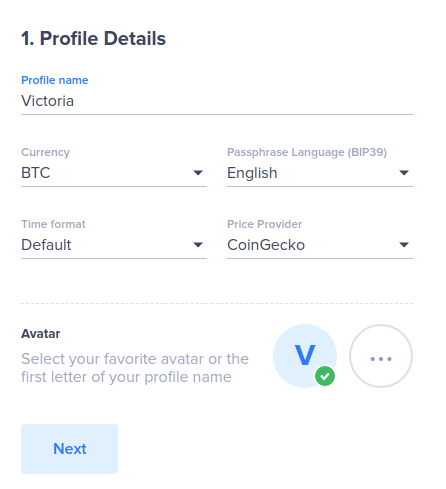
\includegraphics[width=6cm,height=7cm]{figuras/wallet_2.png}}
	\caption{Detalles del perfil}
	\label{fig:wallet-2}
\end{figure}

En el siguiente paso aparece un menú con las posibles redes, \textit{mainnet} y \textit{devnet}. Sin embargo, si se desea usar la red \textit{testnet} es necesario crearla pulsando nueva red. Los campos a rellenar son el nombre, una breve descripción y la dirección del servidor con el puerto de la API, \texttt{http:/GENESIS\_NODE\_IP:API\_PORT}, figura \ref{fig:wallet-3}.

\begin{figure}[H]
	\centering
	\tcbox[colback=white, colframe=codegray]{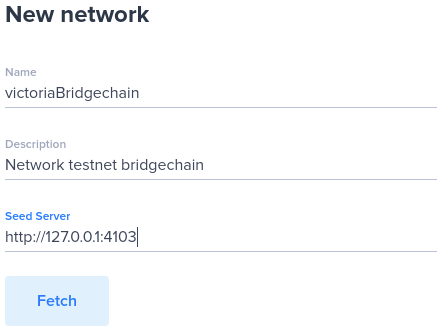
\includegraphics[width=6cm,height=5cm]{figuras/wallet_3.png}}
	\caption{Configuración de la nueva red}
	\label{fig:wallet-3}
\end{figure}

\newpage
Cuando se ha creado la red aparece una pantalla con los detalles de la misma donde debemos de cambiar la dirección por defecto del \textit{explorer} y poner \texttt{http://GENESIS\_NODE\_IP:EXPLORER\_PORT}. También se pueden cambiar el nombre de los Tokens y el símbolo. Una vez realizados los cambios, guardamos la red, figura \ref{fig:wallet-4-5}.\\

\begin{figure}[H]
	\centering
	\begin{minipage}{0.4\textwidth}
		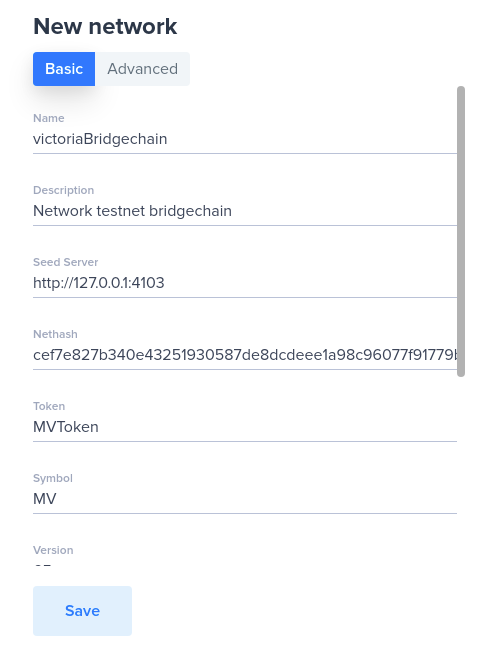
\includegraphics[width=6.5cm,height=8.5cm]{figuras/wallet_4.png}
	\end{minipage}\vfill
	\begin{minipage}{0.38\textwidth}
		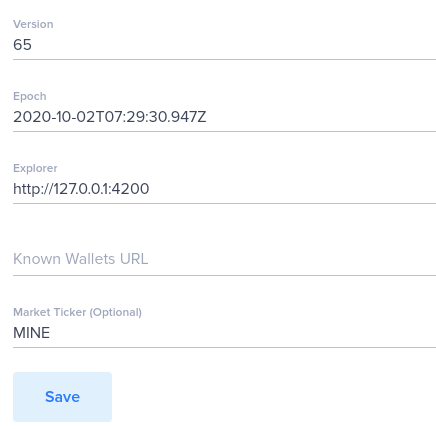
\includegraphics[width=6.3cm,height=8.5cm]{figuras/wallet_5.png}	
	\end{minipage}
	\caption{Detalles de la nueva red}
	\label{fig:wallet-4-5}
\end{figure}

\newpage
Se selecciona la red recien creada, \texttt{victoriaBridgechain} y se avanza al siguiente paso, figura \ref{fig:wallet-6}.\\

\begin{figure}[H]
	\centering
	\tcbox[colback=white, colframe=codegray]{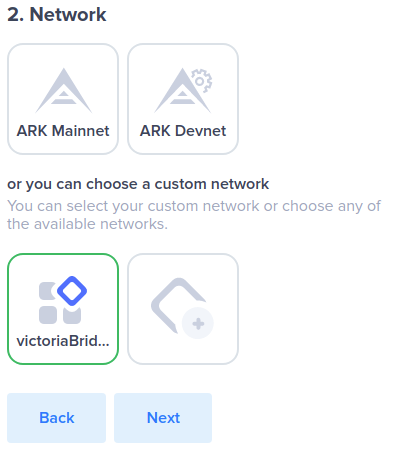
\includegraphics[width=6cm,height=7cm]{figuras/wallet_6.png}}
	\caption{Selección de la red}
	\label{fig:wallet-6}
\end{figure}

Para acabar con la creación del usuario, se tiene la opción de personalizar los colores de la interfaz de usuario o cambiar al tema de noche, figura \ref{fig:wallet-7}.\\

\begin{figure}[H]
	\centering
	\tcbox[colback=white, colframe=codegray]{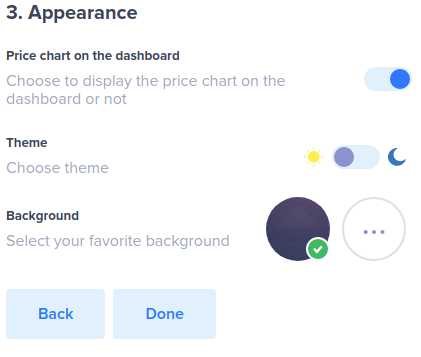
\includegraphics[width=6cm,height=6cm]{figuras/wallet_7.png}}
	\caption{Personalización del diseño de la interfaz}
	\label{fig:wallet-7}
\end{figure}

\newpage
Es necesario conectar la aplicación con la \textit{blockchain}, para que salga la cantidad de dinero inicial. Pulsando en el panel lateral izquierdo en \texttt{Network}, se accede a la configuración de la red y pulsando en \texttt{Connect custom peer} obtenemos la figura \ref{fig:wallet-11-12}. Rellenamos los campos con \texttt{http://GENESIS\_NODE\_IP} y con el \texttt{API\_PORT}. Cuando se conecte hay que refrescar la página para que se actualice el monedero con el dinero.

\begin{figure}[H]
	\centering
	\begin{minipage}{0.3\textwidth}
		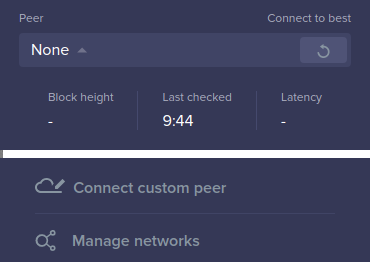
\includegraphics[width=6cm,height=5.5cm]{figuras/wallet_11.png}
	\end{minipage}\hfill
	\begin{minipage}{0.5\textwidth}
		\tcbox[colback=white, colframe=codegray]{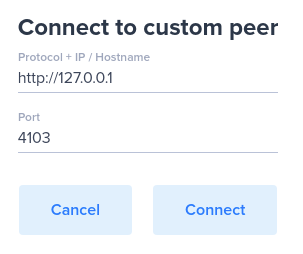
\includegraphics[width=5cm,height=5cm]{figuras/wallet_12.png}}
	\end{minipage}
	\caption{Configuración de la conexión peer}
	\label{fig:wallet-11-12}
\end{figure}

La primera vez que se entra al usuario es necesario importar el monedero que se ha creado durante la instalación de la \textit{blockchain}, pulsando en la esquina superior derecha en \texttt{Import Wallet}. No es necesario rellenar los dos campos, se puede importar el monedero introduciendo solamente la \textit{passphrase}, figura \ref{fig:wallet-8}.

\begin{figure}[H]
	\centering
	\tcbox[colback=white, colframe=codegray]{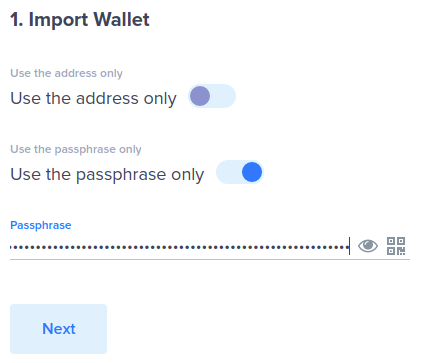
\includegraphics[width=6cm,height=6cm]{figuras/wallet_8.png}}
	\caption{Importar monedero}
	\label{fig:wallet-8}
\end{figure}

Si se desea se puede poner contraseña al monedero, haciéndolo más seguro, en el ejemplo no se van a poner contraseña a ninguno de los monederos, figura \ref{fig:wallet-9}.\\

\begin{figure}[H]
	\centering
	\tcbox[colback=white, colframe=codegray]{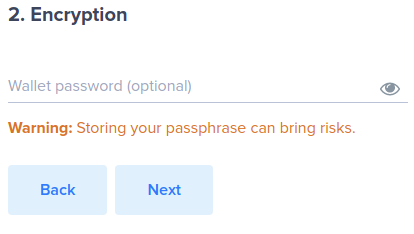
\includegraphics[width=6cm,height=3.8cm]{figuras/wallet_9.png}}
	\caption{Encriptación el monedero}
	\label{fig:wallet-9}
\end{figure}

Finalmente, hay que ponerle nombre al monedero, para diferenciarlo de otros monederos y saber cual es el que contiene la cantidad inicial, el nombre que se le va a poner es \texttt{MainWallet}, figura \ref{fig:wallet-10}.\\

\begin{figure}[H]
	\centering
	\tcbox[colback=white, colframe=codegray]{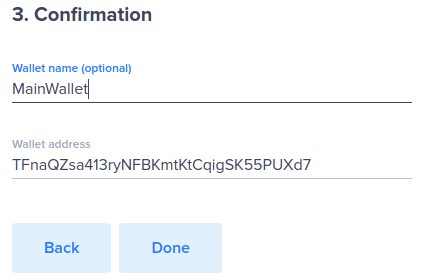
\includegraphics[width=6cm,height=5cm]{figuras/wallet_10.png}}
	\caption{Confirmación para crear el monedero}
	\label{fig:wallet-10}
\end{figure}



\newpage
Para realizar transacciones y poder probar el algoritmo, es necesario crear otro monedero y realizar transacciones entre ambos. De esta forma, hay que acceder a la sección \texttt{My wallets} y pulsar \texttt{Create Wallet}. El primer paso es introducir el nombre del monedero, figura \ref{fig:wallet-13}.\\
 
\begin{figure}[H]
	\centering
	\tcbox[colback=white, colframe=codegray]{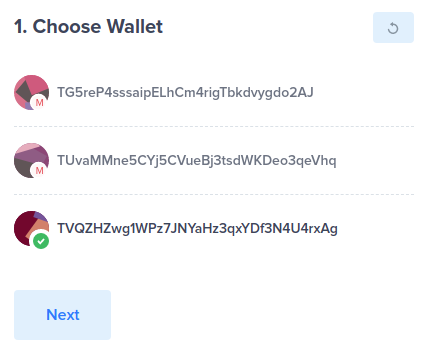
\includegraphics[width=7cm,height=6.5cm]{figuras/wallet_13.png}}
	\caption{Selección de la dirección del nuevo monedero}
	\label{fig:wallet-13}
\end{figure}

La figura \ref{fig:wallet-14} muestra la \textit{passphrase} del monedero. Esta \textit{passphrase} hay que guardarla, tal y como se hizó con la \textit{passphrase} de monedero importado, pues será necesaria para realizar transacciones posteriormente.\\

\begin{figure}[H]
	\centering
	\tcbox[colback=white, colframe=codegray]{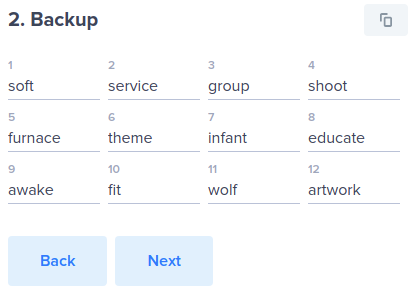
\includegraphics[width=6.5cm,height=5cm]{figuras/wallet_14.png}}
	\caption{\textit{Passphrase} o clave privada del monedero}
	\label{fig:wallet-14}
\end{figure}

\newpage
La verificación de la \textit{passphrase} se hace introduciendo tres palabras, la número tres, seis y nueve, si se desea se puede realizar la verifiación introduciendo todas las palabras, figura \ref{fig:wallet-15}.\\

\begin{figure}[H]
	\centering
	\tcbox[colback=white, colframe=codegray]{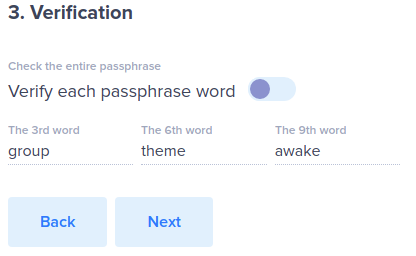
\includegraphics[width=7cm,height=5cm]{figuras/wallet_15.png}}
	\caption{Verificación de la \textit{passphrase}}
	\label{fig:wallet-15}
\end{figure}

Si se desea se puede poner contraseña al monedero, en el ejemplo no es necesario, figura \ref{fig:wallet-16}.\\

\begin{figure}[H]
	\centering
	\tcbox[colback=white, colframe=codegray]{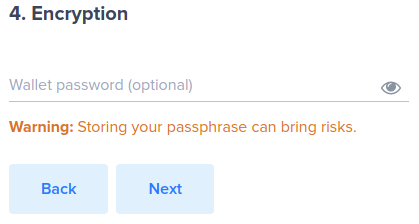
\includegraphics[width=7cm,height=5cm]{figuras/wallet_16.png}}
	\caption{Encriptación del monedero}
	\label{fig:wallet-16}
\end{figure}

\newpage

Antes de confirmar la creación del monedero, hay que introducir el nombre del mismo, \texttt{Second Wallet}, para hacer referencia a que no tendrá ningún token hasta que no reciba una transferencia, figura \ref{fig:wallet-17}.\\

\begin{figure}[H]
	\centering
	\tcbox[colback=white, colframe=codegray]{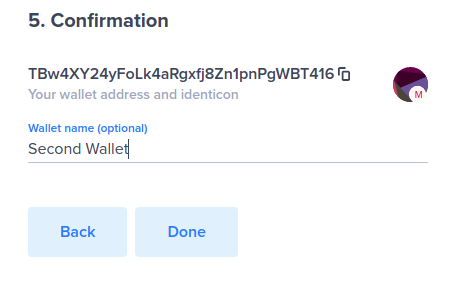
\includegraphics[width=7cm,height=5cm]{figuras/wallet_17.png}}
	\caption{Confirmación para crear el segundo monedero}
	\label{fig:wallet-17}
\end{figure}

A la página principal, donde aparecen los monederos del usuario, se accede pulsando en el panel de la izquierda el símbolo del monedero, sección \texttt{My Wallets}, figura \ref{fig:wallet-princi}. Se puede observar que el usuario en el que nos encontramos se llama ``Victoria'', este contiene dos monederos \texttt{Main Wallet}, con $21.000.000,00$MV y \texttt{Second Wallet}, con $0,00$MV.\\

\begin{figure}[H]
	\centering
	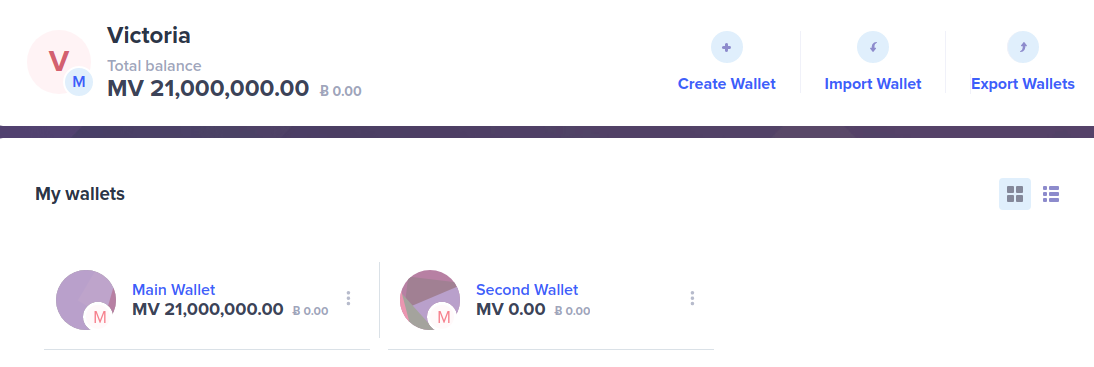
\includegraphics[width=13cm,height=5cm]{figuras/wallet_panel.png}
	\caption{Página principal con los monederos}
	\label{fig:wallet-princi}
\end{figure}

Pulsando en cada uno de los monederos se accede a dicho monedero. Para realizar la primera transacción hay que pulsar en \texttt{Main Wallet} y posteriormente pulsar en la esquina superior derecha \texttt{sent}, figura \ref{fig:transfer}.\\

\begin{figure}[H]
	\centering
	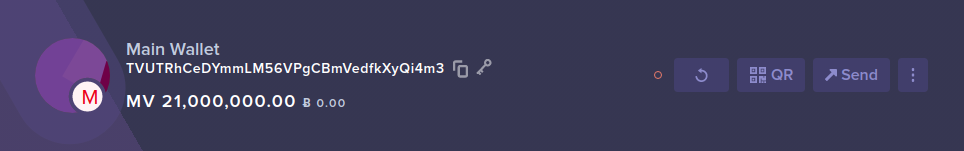
\includegraphics[width=13cm,height=2cm]{figuras/transfer.png}
	\caption{Botón enviar}
	\label{fig:transfer}
\end{figure}

Entonces aparecerá un pantalla emergente para introducir los campos necesarios para realizar la transacción, figura \ref{fig:wallet-18}. Algunos de esos campos son el receptor de la transacción, en el ejemplo se ha enviado al otro monedero anteriormente creado, la cantidad de MVTokens a enviar, un mensaje para el receptor y la clave privada del monedero.

\begin{figure}[H]
	\centering
	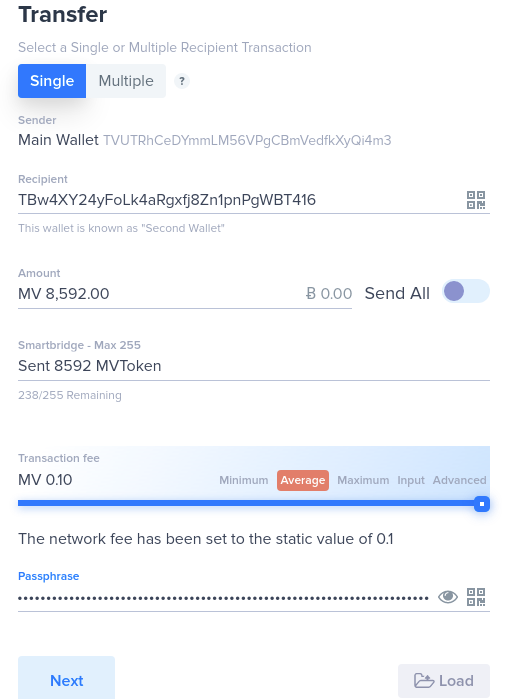
\includegraphics[width=6.5cm,height=10cm]{figuras/wallet_18.png}
	\caption{Realizar transferencia}
	\label{fig:wallet-18}
\end{figure}

Después hay que confirmar la transacción, además se pueden comprobar los datos de la transacción y si fuese necesario es pueden modificar, figura \ref{fig:wallet-19}. También existe la opción de almacenar los datos de la transacción por si en el futuro se desee volver a hacer la misma transacción y no tener que poner otra vez todos los datos. Así en el paso anterior habrá que pulsar \texttt{load} y cargar el archivo con la información de la transacción.

\begin{figure}[H]
	\centering
	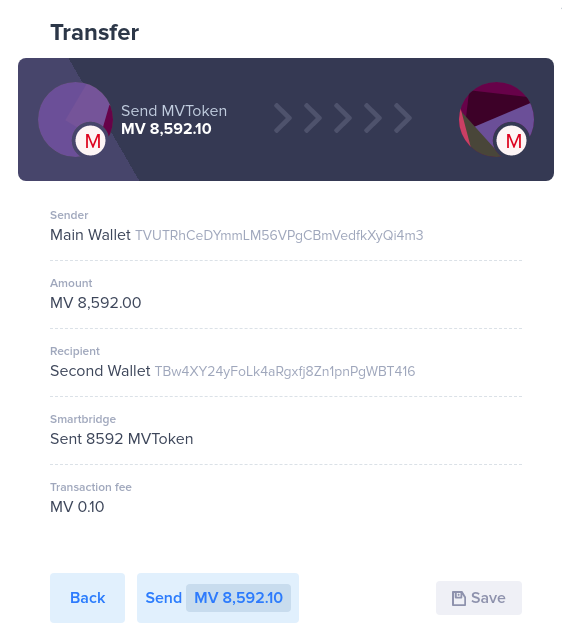
\includegraphics[width=8.5cm,height=10cm]{figuras/wallet_19.png}
	\caption{Confirmación de la transaferencia}
	\label{fig:wallet-19}
\end{figure}

En el modenero desde donde se ha realizado la transacción, se puede ver que se ha creado una nueva entrada en la lista de transacciones, figura \ref{fig:wallet-20}.

\begin{figure}[H]
	\centering
	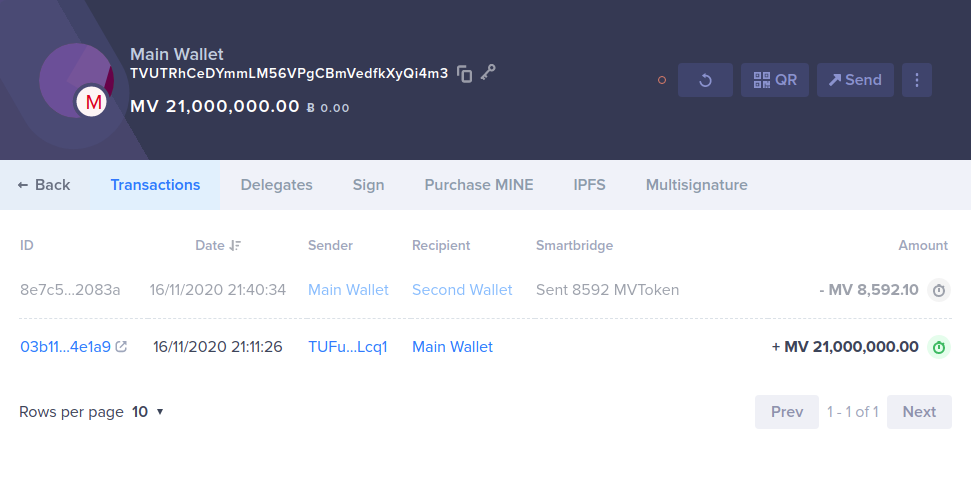
\includegraphics[width=12cm,height=6cm]{figuras/wallet_20.png}
	\caption{Comprobación de que se ha enviado la transaferencia}
	\label{fig:wallet-20}
\end{figure}



%\begin{lstlisting}[language=Bash,caption=Instalación \textit{blockchain}. Parte III, label=cod:suma-cuerpo, style=Consola]

%\end{lstlisting}

\newpage

\section{Visualización de los datos con el Explorer}

Se accede a los logs de la cadena de bloques, a través de la terminal con el comando \texttt{pm2 log}. En la misma terminal se obtendrá una vista similar a la siguiente figura \ref{fig:explorer-1} donde en primer lugar se muestran las salidas de las funciones firma y verificación de UOV, con la firma y el resultado de la validación de la misma, respectivamente. Además del log de la propia \textit{blockchain} indicando que el bloque se ha creado con éxito, en este caso se ha creado el bloque $63372384328353607$. Ha de notarse que la firma del bloque es un vector de vectores con componentes en $\mathds{F}_2$ y que lo que se envía es dicho vector en hexadecimal, por tanto la firma modificada siempre empezará por $5b5b$ que corresponde a los caracteres $[[$.

\begin{figure}[H]
	\centering
	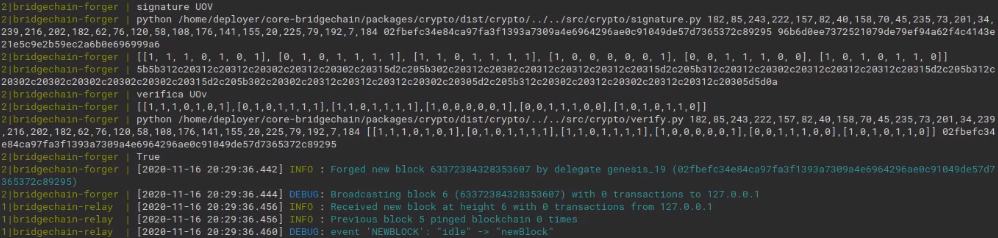
\includegraphics[width=12cm,height=3cm]{figuras/explorer_1.png}
	\caption{Logs de la cadena de bloques}
	\label{fig:explorer-1}
\end{figure}

En el \textit{explorer} de ARK si se accede a \texttt{Lastest Blocks} aparecerán los últimos bloques creados, figura \ref{fig:explorer-2}.

\begin{figure}[H]
	\centering
	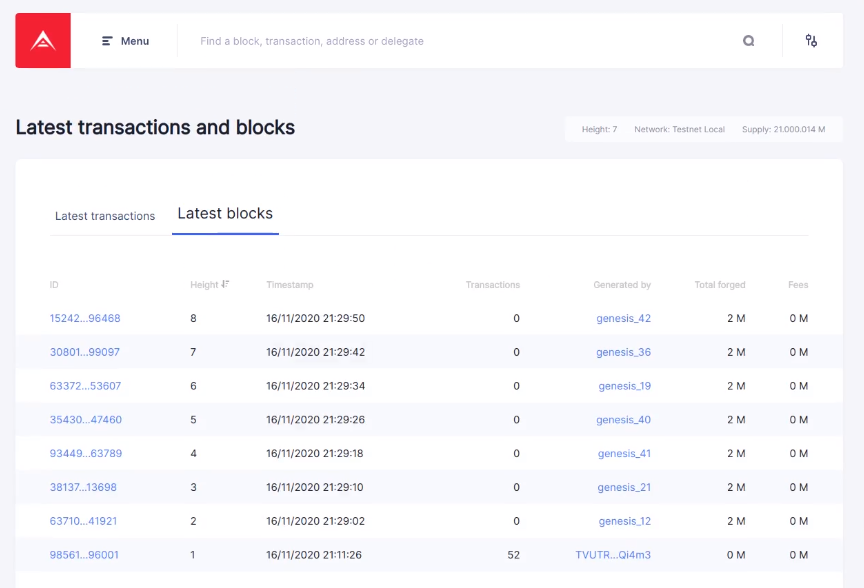
\includegraphics[width=12.5cm,height=8cm]{figuras/explorer_2.png}
	\caption{Vista del \textit{explorer} con los últimos bloques creados}
	\label{fig:explorer-2}
\end{figure}

\newpage
En la misma página se busca el bloque deseado por el ID $63372384328353607$ para ver más información sobre él, figura \ref{fig:explorer-3}.\\

\begin{figure}[H]
	\centering
	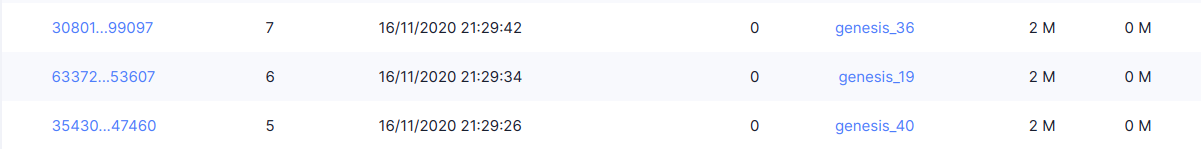
\includegraphics[width=12.5cm,height=1.8cm]{figuras/explorer_3.png}
	\caption{Bloques anterior y posterior del bloque con ID $63372384328353607$}
	\label{fig:explorer-3}
\end{figure}

La figura \ref{fig:explorer-4} muestra toda la información referente al bloque, como el número de transacciones que almacena, el número de confirmaciones por parte de los delegados, la hora a la que se ha generado el bloque o el nombre del delegado que lo ha generado. En la parte superior derecha hay dos botones \texttt{Previous block} y \texttt{Next block}, para acceder al bloque anterior y al bloque siguiente, respectivamente.\\

\begin{figure}[H]
	\centering
	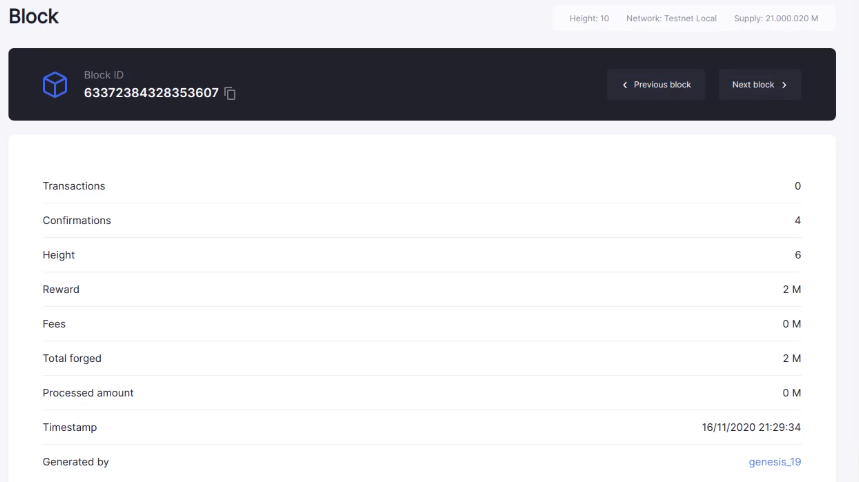
\includegraphics[width=12cm,height=6.5cm]{figuras/explorer_4.png}
	\caption{Información del bloque con ID $63372384328353607$, visto en el \textit{explorer}}
	\label{fig:explorer-4}
\end{figure}

Mientras la información que se puede ver del bloque desde la API es un poco más detallada, el ID del bloque, el ID del bloque anterior, el \textit{hash} del bloque, que delegado ha generado el bloque tanto el nombre como la dirección, la firma del bloque, las confirmaciones y la hora a la que se ha generado, figura \ref{fig:explorer-5}. Se puede comprobar que la firma del bloque comienza por $5b5b$ que es la firma modificada.\\

\begin{figure}[H]
	\centering
	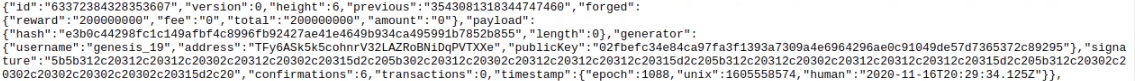
\includegraphics[width=14.7cm,height=1.4cm]{figuras/explorer_5.png}
	\caption{Información del bloque con ID $63372384328353607$, visto en la API}
	\label{fig:explorer-5}
\end{figure}

Finalmente, se puede comprobar que coinciden los bloques mostrados en el \textit{explorer}, figura \ref{fig:explorer-3}, con los de la API. Esto es, ver en la información del siguiente bloque $3080127205067599097$ que se ha creado, que el identificador del bloque anterior es $63372384328353607$, figura \ref{fig:explorer-6}.\\

\begin{figure}[H]
	\centering
	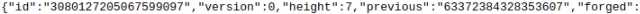
\includegraphics[width=13cm,height=0.4cm]{figuras/explorer_6.png}
	\caption{Información del bloque anterior al bloque $63372384328353607$, visto desde la API}
	\label{fig:explorer-6}
\end{figure}


\newpage







